\section{Estendere HD Viz}
    \subsection{Descrizione}
    HD Viz è un prodotto open source ed in quanto tale ogni utente può modificare, estendere e ridistribuire la propria versione del codice sorgente. In questa sezione è possibile consultare le norme e le modalità attraverso le quali si può estendere e modificare il progetto HD Viz.
    \subsection{Contribuire al progetto principale}
    Il progetto principale è gestito dai componenti del gruppo \textit{HD Viz}, e si può trovare al seguente repository Github: \url{https://github.com/CodeOfDutyJS/hdviz}.
    Il gruppo \textit{HD Viz} si riserva il diritto di approvare e verificare ogni modifica apportata al progetto principale.
        \subsubsection{Diagramma di attività di modifica e/o estensione al progetto}
        Il seguente diagramma illustra l'attività di modifica e/o estensione del progetto:
        \\
        \\
        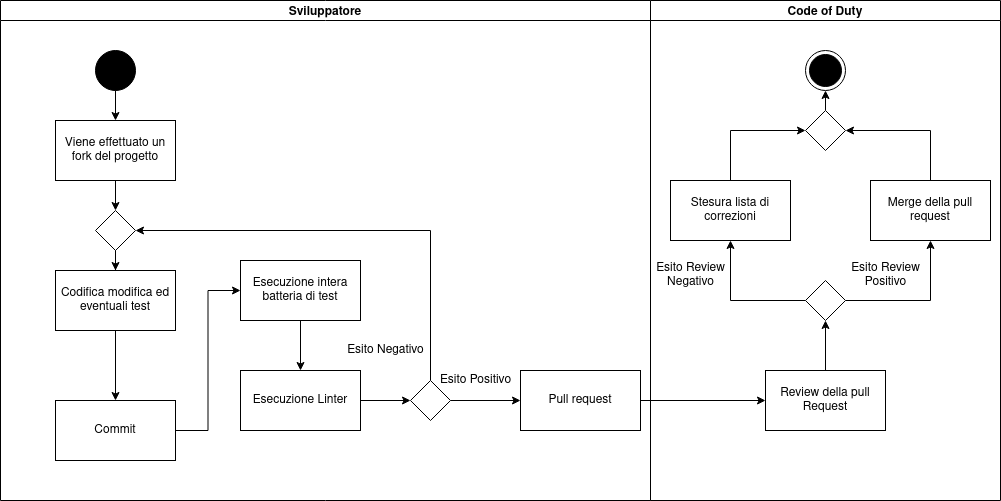
\includegraphics[width=1\textwidth]{source/img/estensione_progetto.png}
        \subsubsection{Descrizione attività di modifica e/o estensione al progetto}
        L'attività di modifica e/o estensione al progetto si svolge nel seguente modo:
        \begin{itemize}
            \item lo sviluppatore esegue un fork del progetto;
            \item codifica la modifica;
            \item codifica eventuali test necessari;
            \item esegue il commit della modifica;
            \item esegue L'intera batteria di test;
            \item esegue il linter;
            \item nel caso sia i test che il linter diano risultato positivo esegue una pull request;
            \item un membro del gruppo \textit{HD Viz} esegue la review della pull request;
            \item in caso la review dia esito negativo viene stesa una lista di correzioni da eseguire;
            \item in caso la review dia esito positivo viene approvata la pull request.
        \end{itemize}
        \subsubsection{Issue}
        Alla pagina Github di \textit{HD Viz} è possibile trovare una board con tutte le Issue attive in un dato momento. La gestione delle Issue stesse è riservata al gruppo \textit{HD Viz}, ma chiunque può contribuire suggerendo miglioramenti e correzioni, o segnalando eventuali bug. 
        \subsubsection{Effettuare il fork}
        Per effettuare il fork del progetto è sufficiente andare alla pagina Github e cliccare sul pulsante "fork" in alto a destra.
        \subsubsection{Pull Request}
        Le pull request sono soggette alle seguenti norme:
        \begin{itemize}
            \item ogni pull request deve contenere una descrizione estensiva delle modifiche e correzioni apportate al progetto, se con la pull request vengono risolte delle Issue si deve porre un riferimento alle stesse;
            \item ogni pull request è soggetta alle regole interne di \textit{Code of Duty} per quanto riguarda il processo di verifica e validazione;
            \item ogni pull request può essere commentata da qualsiasi utente;
            \item il gruppo \textit{Code of Duty} si riserva il diritto ultimo di approvare o chiudere una pull request, in ogni caso una modifica allo stato della pull request deve essere giustificata con un commento;
            \item il gruppo \textit{Code of Duty} non assicura alcun limite di tempo al processo di review.
        \end{itemize}
        \subsubsection{Stesura dei test}
        La stesura dei test viene riconosciuta dal gruppo \textit{Code of Duty} come buona pratica per la stesura di codice di qualità. Chiunque voglia contribuire scrivendo test per l'applicazione o per testare la propria estensione e/o modifica del codice deve:
        \begin{itemize}
            \item usare il framework jest
            \item seguire le convenzioni del gruppo sul nome dei file di test, cioè usare la seguente convenzione per i nomi dei file:
            \begin{verbatim}
                nomeClasse.spec.js
            \end{verbatim}
            dove nomeClasse è il nome della classe da testare;
            \item porre i file di test nella cartella corrispondente nell'albero di test, ad esempio se si vuole testare
            \begin{verbatim}
                hdviz/client/src/d3/newVisualization.js
            \end{verbatim}
            inserire il test in:
            \begin{verbatim}
                hdviz/client/src/test/d3/newVisualization.spec.js
            \end{verbatim}.
        \end{itemize}
    \subsection{Usare HD Viz come base per un altro progetto}
    HD Viz è un progetto open-source, chiunque può usare il codice del progetto in parte o nella sua interezza e ridistribuirlo gratuitamente o dietro pagamento.
    \subsection{Aggiungere una visualizzazione}
    Per aggiungere una visualizzazione creare un nuovo file .js in:
    \begin{verbatim}
        client/src/model/d3
    \end{verbatim}
    all'interno del file creare una funzione contenente il codice d3 da eseguire. Per convenzione d3 all'interno del progetto viene importato con:
    \begin{verbatim}
        import * as d3 from 'd3';
    \end{verbatim}
    \textit{HD Viz} contiene un unico elemento svg con id \#area, questo è utile per la manipolazione del DOM in quanto rende l'svg selezionabile con un sola istruzione d3:
    \begin{verbatim}
        const svg = d3.select('#area');
    \end{verbatim}
        \subsubsection{Inserire la nuova visualizzazione}
        Ogni visualizzazione deve essere associata ad un modello. Ogni modello implementa la funzione  \texttt{getPreparedDataset()}, che ritorna i dati alla visualizzazione. Se si vuole sfruttare un modello già esistente è necessario creare una nuova classe che eredita dal modello e reimplementare \texttt{getPreparedDataset()} con i dati necessari alla propria visualizzazione. Successivamente perché la visualizzazione sia disponibile e selezionabile dalla UI è sufficiente aggiungere un \texttt{VisualizationType} nel \texttt{VisualizationCollector}, in questo modo:
        \begin{verbatim}
            VisualizationCollector.addVisualization({
              id: 'myviz',
              label: 'My Visualization',
              model: new MyVisualizationModel(),
              visualization: myVisualization,
              options: { distance: true },
            });
        \end{verbatim}
        
        Per convenzione questa porzione di codice viene inserita all'interno del file del suo corrispondente \texttt{VisualizationModel}, fuori dallo scope della classe.
        
        I parametri che vengono passati a \texttt{.addVisualization()} sono:
        \begin{itemize}
            \item \textbf{id}: id univoco per la visualizzazione;
            \item \textbf{label}: testo che viene mostrato nella UI per la selezione della visualizzazione;
            \item \textbf{model}: l'oggetto del nuovo modello di visualizzazione;
            \item \textbf{visualization}: la funzione della nuova visualizzazione;
            \item \textbf{options}: le opzioni che la UI deve visualizzare, nell'esempio distance, quindi verrà visualizzata la selezione del tipo di distanza.
        \end{itemize}
    
        Una volta aggiunta la visualizzazione al \texttt{VisualizationCollector} è necessario importare il nuovo file all'interno del file index.js nella cartella VisualizationModels.
        
        \subsubsection{Pratiche usate dal gruppo usando d3}
            Questa sezione contiene pratiche che pur non essendo convenzionate sono considerate dal gruppo utili per la creazione di visualizzazioni d3.
            \myparagraph{Utilizzo di tag g}
            Pur non essendo strettamente necessario creare dei gruppi all'interno dei quali inserire (o come lo definisce d3 "appendere") gli elementi sui quali andrà effettivamente eseguito il data binding si rivela molto utile a livello organizzativo e gestionale, in particolare le operazioni di trasformazioni applicate all'intero gruppo si riflettono su tutti i suoi membri, mentre quelle all'interno del gruppo sono relative alla trasformazione "padre".
            \myparagraph{Resize e dimensioni dell'svg}
            Il resize dello schermo può essere gestito molto semplicemente in particolare il modo per inserire una callback all'evento onresize è il seguente:
            \begin{verbatim}
            d3.select('window')
              .on('resize', callback);
            \end{verbatim}
            dove l'utente può inserire una qualsiasi funzione al posto di callback. Viene da se che per gestire l'evento di resize si dovrà disegnare di nuovo la visualizzazione. Quindi si rende necessario "pulire" lo schermo con:
            \begin{verbatim}
                d3.select('#area').selectAll('*').remove();
            \end{verbatim}
            e poi successivamente a richiamare la propria funzione di visualizzazione.
            Si rende però altresì necessario esprimere le dimensioni della visualizzazione rispetto alle dimensioni dell'svg. Queste possono essere trovate con:
            \begin{verbatim}
                const { width, height } = svg.node().getBoundingClientRect();
            \end{verbatim}
    \subsection{Aggiungere un modello}
    Le classi modello vengono aggiunte all'interno di:
    \begin{verbatim}
        client/src/model/VisualizationModels
    \end{verbatim}
    solitamente la classe di modello viene chiamata come la funzione di visualizzazione con l'aggiunta di Model, ad esempio:
    \begin{verbatim}
        LinearProjection
    \end{verbatim}
    diventa:
    \begin{verbatim}
        LinearProjectionModel
    \end{verbatim}
    Si deve ereditare da \texttt{VisualizationModel}. Si deve implementare il metodo \texttt{getPreparedDataset()}, restituendo un oggetto contenente i dati da passare alla funzione di visualizzazione.
    
    Il metodo \texttt{getPreparedDataset()} per convenzione può avere in input delle opzioni, come la funzione di distanza o di normalizzazione da utilizzare.
    
    se si vuole ricevere in input queste opzioni è necessario riceverle come oggetto:
    
    \begin{verbatim}
        getPreparedDataset({ distanceFn, normalizeFn }){
            ...
        }
    \end{verbatim}
    Per convenzione se si vuole richiedere la funzione di distanza è necessario aggiungere \texttt{distanceFn} mentre per la funzione di normalizzazione è necessario aggiungere \texttt{normalizeFn}.
    
    \subsection{Aggiungere una legenda}
    Vengono fornite due funzioni, dentro \texttt{client/src/model/d3}
    chiamate \texttt{drawTargetLegend()} e \texttt{drawColorScale()}.
    \texttt{drawTargetLegend()} si occupa di disegnare la leggenda dei target, assegna colore e testo ad ogni valore differente di target, ed ha la seguente firma:
    \begin{verbatim}
        function drawTargetLegend(color, target, x, y, height, width) 
    \end{verbatim}
    dove:
    \begin{itemize}
        \item \texttt{color} è la funzione di colore d3 usata per assegnare i colori ai target, basta passare la stessa funzione usata nella funzione di visualizzazione;
        \item \texttt{target} è un array contenente gli oggetti target, si può passare direttamente\\\texttt{this.dataModel.getTargetColumns()} dal modello;
        \item \texttt{x} è la coordinata x della legenda;
        \item \texttt{y} è la coordinata y della legenda;
        \item \texttt{height} è l'altezza della legenda;
        \item \texttt{width} è la larghezza della legenda.
    \end{itemize}
    mentre \texttt{drawColorScale()} ha la seguente firma:
    \begin{verbatim}
        function drawColorScale(color, range, x, y, width, height, name)
    \end{verbatim}
    e si occupa di disegnare un range di colori con la scala associata. i parametri sono gli stessi ad eccezione di:
    \begin{itemize}
        \item \texttt{range}: un array nella forma [min, max] dove min e max sono gli estremi del range di visualizzazione, alternativamente è possibile passare un array contenente tutti i valori della visualizzazione;
        \item \texttt{name}: una stringa rappresentante il nome della scala.
    \end{itemize}